\chapter{Teoria de nombres}

\index{teoria de nombres}

La \key{teoria de nombres} és una branca de les matemàtiques que estudia
els nombres enters. La teoria dels nombres és un camp fascinant,
perquè moltes qüestions que impliquen nombres enters són molt difícils
de resoldre encara que a primera vista semblin senzilles.

Com a exemple, considereu l'equació següent:
\[x^3 + y^3 + z^3 = 33\]
És fàcil trobar tres nombres reals $x$, $y$ i $z$ que compleixin
l'equació. Per exemple, podem triar
\[
\begin{array}{lcl}
x = 3, \\
y = \sqrt[3]{3}, \\
z = \sqrt[3]{3}.\\
\end{array}
\]
Tanmateix, és un problema obert en teoria de nombres si hi ha tres
\emph{enters} $x$, $y$ i $z$ que satisfacin l'equació \cite{bec07}.

En aquest capítol, ens centrarem en els conceptes bàsics i algorismes
de la teoria dels nombres. Al llarg del capítol, assumirem que tots
els nombres són enters si no s'indica el contrari.

\section{Nombres primers i factors}

\index{divisibilitat} \index{factor} \index{divisor}

Un nombre $a$ s'anomena \key{factor} o \key{divisor} d'un nombre $b$
si $a$ divideix $b$. Si $a$ és un factor de $b$, escrivim $a \mid b$,
i en cas contrari escrivim $a \nmid b$. Per exemple, els factors de 24
són 1, 2, 3, 4, 6, 8, 12 i 24.

\index{nombre primer} \index{descomposició en nombres primers}

Un nombre $n>1$ és un nombre \key{primer} si els seus únics factors
positius són 1 i $n$. Per exemple, 7, 19 i 41 són primers, però 35 no
és primer, perquè $5 \cdot 7 = 35$. Per a cada nombre $n>1$, hi ha una
\key{factorització en nombres primers} única
\[ n = p_1^{\alpha_1} p_2^{\alpha_2} \cdots p_k^{\alpha_k},\]
on $p_1,p_2,\ldots,p_k$ són nombres primers diferents i
$\alpha_1,\alpha_2,\ldots,\alpha_k$ són nombres positius. Per exemple,
la factorització en nombres primers per a 84 és
\[84 = 2^2 \cdot 3^1 \cdot 7^1.\]


El \key{nombre de factors} d'un nombre $n$ és
\[\tau(n)=\prod_{i=1}^k (\alpha_i+1),\]
perquè per a cada $p_i$ primer, hi ha $\alpha_i+1$ maneres de triar
quantes vegades apareix en el factor. Per exemple, el nombre de
factors de 84 és $\tau(84)=3 \cdot 2 \cdot 2 = 12$. Els factors són 1,
2, 3, 4, 6, 7, 12, 14, 21, 28, 42 i 84.

La \key{suma de factors} de $n$ és
\[\sigma(n)=\prod_{i=1}^k (1+p_i+\ldots+p_i^{\alpha_i}) = \prod_{i=1}^k \frac{p_i^{a_i+1}-1}{p_i-1},\]
on aquesta última fórmula es basa en la fórmula de la progressió
geomètrica. Per exemple, la suma de factors de 84 és
\[\sigma(84)=\frac{2^3-1}{2-1} \cdot \frac{3^2-1}{3-1} \cdot \frac{7^2-1}{7-1} = 7 \cdot 4 \cdot 8 = 224.\]


El \key{producte de factors} de $n$ és
\[\mu(n)=n^{\tau(n)/2},\]
perquè podem formar $\tau(n)/2$ parells a partir dels factors,
cadascun amb el producte $n$. Per exemple, els factors de 84
produeixen els parells $1 \cdot 84$, $2 \cdot 42$, $3 \cdot 28$, etc.,
i el producte dels factors és $\mu(84)=84^6=351298031616 $.

\index{nombre perfecte}

Un nombre $n$ s'anomena \key{perfecte} si $n=\sigma(n)-n$, és a
dir, $n$ és igual a la suma dels seus factors entre $1$ i $n-1$. Per
exemple, 28 és un nombre perfecte, perquè $28=1+2+4+7+14$.

\subsubsection{Infinits nombres primers}

És fàcil demostrar que hi ha una quantitat infinita de nombres primers. Si
el nombre de primers fos finit, podríem construir un conjunt
$P=\{p_1,p_2,\ldots,p_n\}$ que contingués tots els primers. Per
exemple, $p_1=2$, $p_2=3$, $p_3=5$, etc. Tanmateix, utilitzant $P$,
podríem formar un nou nombre primer
\[p_1 p_2 \cdots p_n+1\]
més gran que tots els elements de $P$. Això és una contradicció, i per tant
hi ha infinits nombres primers.

\subsubsection{Densitat dels nombres primers}

La densitat de nombres primers és la freqüència amb que els nombres
primers apareixen entre tots els nombres. Sigui $\pi(n)$ la quantitat
de nombres primers entre $1$ i $n$. Per exemple, $\pi(10)=4$, perquè
hi ha 4 nombres primers entre $1$ i $10$: 2, 3, 5 i 7.

És possible demostrar que
\[\pi(n) \approx \frac{n}{\ln n},\]
el que vol dir que els nombres primers són força freqüents. Per
exemple, la quantitat de nombres primers entre $1$ i $10^6$ és
$\pi(10^6)=78498$ i $10^6 / \ln 10^6 \approx 72382$.

\subsubsection{Conjectures}

Hi ha moltes \emph{conjectures} que tenen a veure amb nombres
primers. La majoria de la gent pensa que les conjectures són certes,
però ningú les ha pogut demostrar. Per exemple, les conjectures
següents són famoses:


\begin{itemize}
\index{La conjectura de Goldbach}
\item \key{Conjectura de Goldbach}:
Cada enter parell $n>2$ es pot representar com a
suma $n=a+b$ de manera que tant $a$ com $b$ són primers.
\index{doble primer}
\item \key{Conjectura dels nombres primers bessons}:
Hi ha un nombre infinit de parelles
de la forma $\{p,p+2\}$,
on tant $p$ com $p+2$ són primers.
\index{La conjectura de Legendre}
\item \key{La conjectura de Legendre}:
Sempre hi ha un nombre primer entre els nombres
$n^2$ i $(n+1)^2$, on $n$ és qualsevol nombre enter positiu.
\end{itemize}


\subsubsection{Algorismes bàsics}

Si un nombre $n$ no és primer, es pot representar com a producte $a
\cdot b$, on $a \le \sqrt n$ o $b \le \sqrt n$, de manera que
certament té un factor entre $2$ i $\lfloor \sqrt n \rfloor$. Amb
aquesta observació, podem comprovar si un nombre és primer i trobar la
factorització en primers d'un nombre en temps $O(\sqrt n)$.

La següent funció \texttt{prime} verifica si el nombre donat $n$ és
primer. La funció intenta dividir $n$ per tots els nombres entre $2$ i
$\lfloor \sqrt n \rfloor$, i si cap d'ells divideix $n$, llavors $n$
és primer.


\begin{lstlisting}
bool prime(int n) {
    if (n < 2) return false;
    for (int x = 2; x*x <= n; x++) {
        if (n%x == 0) return false;
    }
    return true;
}
\end{lstlisting}


\noindent La funció \texttt{factors} següent construeix un vector que
conté la factorització en nombres primers de $n$. La funció divideix
$n$ pels seus factors primers i els afegeix al vector. El procés acaba
quan el nombre resultant $n$ no té factors entre $2$ i $\lfloor \sqrt
n \rfloor$. Si $n>1$, és un nombre primer i esdevé l'últim factor.


\begin{lstlisting}
vector<int> factors(int n) {
    vector<int> f;
    for (int x = 2; x*x <= n; x++) {
        while (n%x == 0) {
            f.push_back(x);
            n /= x;
        }
    }
    if (n > 1) f.push_back(n);
    return f;
}
\end{lstlisting}


Tingueu en compte que cada factor primer apareix al vector tantes
vegades com divideix el nombre. Per exemple, $24=2^3 \cdot 3$, de
manera que el resultat de la funció és $[2,2,2,3]$.

\subsubsection{Sedàs d'Eratòstenes}

\index{sedàs d'Eratòstenes}

El \key{sedàs d'Eratòstenes} %\footnote{Eratòstenes (c. 276 aC --
%c. 194 aC) va ser un matemàtic grec.}
és un algorisme de preprocessament que construeix un vector
mitjançant el qual podem comprovar de manera eficient si un nombre
determinat entre $2 \ldots n$ és primer i, si no ho és, troba un
factor primer del nombre.

L'algorisme crea un vector $\texttt{sieve}$, del qual farem servir les
posicions $2, 3, \ldots, n$. El valor $\texttt{sieve}[k]=0$ vol dir
que $k$ és primer, i el valor $\texttt{sieve}[k] \neq 0$ vol dir que
$k$ no és primer i que $\texttt{sieve}[k]$ és un dels seus factors
primers.

L'algorisme itera els nombres $2 \ldots n$ un per un. Sempre que troba
un nou nombre primer $x$, l'algorisme enregistra que els múltiples de
$x$ ($2x,3x,4x,\ldots$) no són primers, ja que $x$ és un divisor.

Per exemple, si $n=20$, el vector resultant és:


\begin{center}
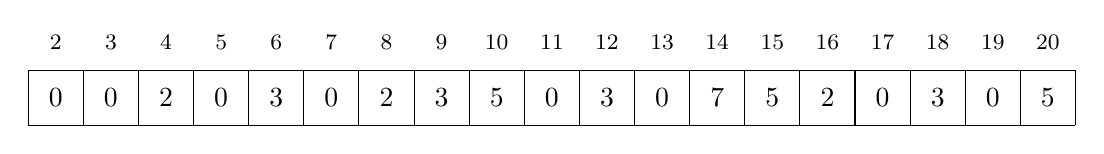
\begin{tikzpicture}[scale=0.7]
\draw (0,0) grid (19,1);

\node at (0.5,0.5) {$0$};
\node at (1.5,0.5) {$0$};
\node at (2.5,0.5) {$2$};
\node at (3.5,0.5) {$0$};
\node at (4.5,0.5) {$3$};
\node at (5.5,0.5) {$0$};
\node at (6.5,0.5) {$2$};
\node at (7.5,0.5) {$3$};
\node at (8.5,0.5) {$5$};
\node at (9.5,0.5) {$0$};
\node at (10.5,0.5) {$3$};
\node at (11.5,0.5) {$0$};
\node at (12.5,0.5) {$7$};
\node at (13.5,0.5) {$5$};
\node at (14.5,0.5) {$2$};
\node at (15.5,0.5) {$0$};
\node at (16.5,0.5) {$3$};
\node at (17.5,0.5) {$0$};
\node at (18.5,0.5) {$5$};

\footnotesize

\node at (0.5,1.5) {$2$};
\node at (1.5,1.5) {$3$};
\node at (2.5,1.5) {$4$};
\node at (3.5,1.5) {$5$};
\node at (4.5,1.5) {$6$};
\node at (5.5,1.5) {$7$};
\node at (6.5,1.5) {$8$};
\node at (7.5,1.5) {$9$};
\node at (8.5,1.5) {$10$};
\node at (9.5,1.5) {$11$};
\node at (10.5,1.5) {$12$};
\node at (11.5,1.5) {$13$};
\node at (12.5,1.5) {$14$};
\node at (13.5,1.5) {$15$};
\node at (14.5,1.5) {$16$};
\node at (15.5,1.5) {$17$};
\node at (16.5,1.5) {$18$};
\node at (17.5,1.5) {$19$};
\node at (18.5,1.5) {$20$};

\end{tikzpicture}
\end{center}


El codi següent implementa el sedàs d'Eratòstenes. El codi assumeix
que cada element de \texttt{sieve} és inicialment zero.


\begin{lstlisting}
for (int x = 2; x <= n; x++) {
    if (sieve[x]) continue;
    for (int u = 2*x; u <= n; u += x) {
        sieve[u] = x;
    }
}
\end{lstlisting}


El bucle intern de l'algorisme s'executa $n/x$ vegades per cada valor
de $x$. Així, el temps d'execució de l'algorisme està limitat per la suma
harmònica
\[\sum_{x=2}^n n/x = n/2 + n/3 + n/4 + \cdots + n/n = O(n \log n).\]


\index{suma harmònica}

De fet, l'algorisme és més eficient, perquè el bucle intern només
s'executa si el nombre $x$ és primer. Es pot demostrar que el temps
d'execució de l'algorisme és $O(n \log \log n)$, una complexitat molt
propera a $O(n)$.

\subsubsection{Algorisme d'Euclides}

\index{màxim comú divisor} \index{mínim comú múltiple} \index{Algorisme d'Euclides}

El \key{màxim comú divisor} (\emph{greatest common divisor}) dels
nombres $a$ i $b$, $\gcd(a,b)$, és el nombre més gran que divideix $a$
i $b$, i el \key{mínim comú múltiple} (\emph{least common multiple})
de $a$ i $b$, $\textrm{lcm}(a,b)$, és el nombre més petit que és
divisible per $a$ i $b$. Per exemple, $\gcd(24,36)=12$ i
$\textrm{lcm}(24,36)=72$.

El màxim comú divisor i el mínim comú múltiple estan connectats de la
següent manera:
\[\textrm{lcm}(a,b)=\frac{ab}{\textrm{gcd}(a,b)}\]


\key{Algorisme d'Euclides}\footnote{Euclides va ser un matemàtic grec
que va viure cap al 300 aC. Aquest és potser el primer algorisme
conegut de la història.} proporciona una manera eficient de trobar el
màxim comú divisor de dos nombres. L'algorisme es basa en la fórmula
següent:
\begin{equation*}
    \textrm{gcd}(a,b) = \begin{cases}
               a        & b = 0\\
               \textrm{gcd}(b,a \bmod b) & b \neq 0\\
           \end{cases}
\end{equation*}


Per exemple, \[\textrm{gcd}(24,36) = \textrm{gcd}(36,24) =
\textrm{gcd}(24,12) = \textrm{gcd}(12,0)=12 .\]

L'algorisme es pot implementar de la següent manera:
\begin{lstlisting}
int gcd(int a, int b) {
    if (b == 0) return a;
    return gcd(b, a%b);
}
\end{lstlisting}


Es pot demostrar que l'algorisme d'Euclides funciona en temps $O(\log
n)$, on $n=\min(a,b)$. El pitjor cas per a l'algorisme és quan $a$ i
$b$ són nombres de Fibonacci consecutius. Per
exemple, \[\textrm{gcd}(13,8)=\textrm{gcd}(8,5)
=\textrm{gcd}(5,3)=\textrm{gcd}(3,2)=\ textrm{gcd}(2,1)=\textrm{gcd}(1,0)=1.\]

\subsubsection{Funció $\varphi$ d'Euler}

\index{coprimer} \index{Funció $\varphi$ d'Euler}

Els nombres $a$ i $b$ són \key{coprimers} si $\textrm{gcd}(a,b)=1$. La \key{funció $\varphi$ (fi) d'Euler} $\varphi(n)$
%\footnote{Euler va presentar aquesta funció el 1763.}
és la quantitat de nombres coprimers amb $n$ entre $1$ i $n$. Per
exemple, $\varphi(12)=4$, perquè 1, 5, 7 i 11 són coprimers amb 12.

El valor de $\varphi(n)$ es pot calcular a partir de la factorització
en primers de $n$ mitjançant la fórmula
\[ \varphi(n) = \prod_{i=1}^k p_i^{\alpha_i-1}(p_i-1). \]
Per exemple, $\varphi(12)=2^1 \cdot (2-1) \cdot 3^0 \cdot
(3-1)=4$. Tingueu en compte que $\varphi(n)=n-1$ si $n$ és primer.

\section{Aritmètica modular}

\index{aritmètica modular}

En l'\key{aritmètica modular}, el conjunt de nombres està limitat de
manera que només s'utilitzen els nombres $0,1,2,\ldots,m-1$, on $m$ és
una constant. Cada nombre $x$ es representa amb el nombre $x \bmod m$:
el residu després de dividir $x$ per $m$. Per exemple, si $m=17$,
llavors $75$ es representa amb $75 \bmod 17 = 7$.

Sovint podem calcular les restes abans de fer càlculs. En particular, es
compleixen les següents fórmules:
\[
\begin{array}{rcl}
(x+y) \bmod m & = & (x \bmod m + y \bmod m) \bmod m \\
(x-y) \bmod m & = & (x \bmod m - y \bmod m) \bmod m \\
(x \cdot y) \bmod m & = & (x \bmod m \cdot y \bmod m) \bmod m \\
x^n \bmod m & = & (x \bmod m)^n \bmod m \\
\end{array}
\]


\subsubsection{Exponenciació modular}

Sovint cal calcular de manera eficient el valor de $x^n \bmod m$. Això
es pot fer en temps $O(\log n)$ amb la recursivitat següent:
\begin{equation*}
    x^n = \begin{cases}
               1        & n = 0\\
               x^{n/2} \cdot x^{n/2} & \text{$n$ is even}\\
               x^{n-1} \cdot x & \text{$n$ is odd}
           \end{cases}
\end{equation*}


És important que, quan $n$ és parell, el valor $x^{n/2}$ només es
calculi una vegada. Això garanteix que la complexitat temporal de
l'algorisme és $O(\log n)$, ja que $n$ sempre es redueix a la meitat
quan és parell.

La funció següent calcula el valor de $x^n \bmod m$:


\begin{lstlisting}
int modpow(int x, int n, int m) {
    if (n == 0) return 1%m;
    long long u = modpow(x,n/2,m);
    u = (u*u)%m;
    if (n%2 == 1) u = (u*x)%m;
    return u;
}
\end{lstlisting}


\subsubsection{Teorema de Fermat i Teorema d'Euler}

\index{Teorema de Fermat} \index{Teorema d'Euler}

El \key{teorema de Fermat} %\footnote{Fermat va descobrir aquest teorema l'any 1640.}
afirma que
\[x^{m-1} \bmod m = 1\]
quan $m$ és primer i $x$ i $m$ són coprimers. Això també implica
\[x^k \bmod m = x^{k \bmod (m-1)} \bmod m.\]
De manera més general, \key{teorema d'Euler} %\footnote{Euler va publicar aquest teorema el 1763.}
afirma que
\[x^{\varphi(m)} \bmod m = 1\]
quan $x$ i $m$ són coprimers. El teorema de Fermat és una conseqüència del
teorema d'Euler, perquè si $m$ és primer, aleshores $\varphi(m)=m-1$.

\subsubsection{Invers modular}

\index{invers modular}

L'invers de $x$ mòdul $m$ és un nombre $x^{-1}$ tal que
\[ x x^{-1} \bmod m = 1. \]
Per exemple, si $x=6$ i $m=17$, aleshores $x^{-1}=3$, ja que $6\cdot3 \bmod 17=1$.

Els inversos modulars es fan servir per dividir nombres mòdul $m$, ja
que divider per $x$ és el mateix que multiplicar per $x^{-1}$. Per
exemple, per avaluar el valor de $36/6 \bmod 17$, podem fer servir la
fórmula $2 \cdot 3 \bmod 17$, ja que $36 \bmod 17 = 2$ i $6^{-1} \bmod
17 = 3 $.

Tanmateix, no sempre existeix un invers modular. Per exemple, si $x=2$
i $m=4$, l'equació
\[ x x^{-1} \bmod m = 1 \]
no es pot resoldre, perquè tots els múltiples de 2 són parells i el
residu no pot ser mai 1 quan $m=4$. Resulta que el valor de
$x^{-1} \bmod m$ es pot calcular exactament quan $x$ i $m$ són coprimers.

Si existeix un invers modular, es pot calcular mitjançant la fórmula
\[
x^{-1} = x^{\varphi(m)-1}.
\]
Si $m$ és primer, la fórmula esdevé
\[
x^{-1} = x^{m-2}.
\]
Per exemple,
\[6^{-1} \bmod 17 =6^{17-2} \bmod 17 = 3.\]


Aquesta fórmula ens permet calcular eficaçment inversos modulars
mitjançant l'algorisme d'exponentació modular. La fórmula es deriva
fent servir el teorema d'Euler. En primer lloc, l'invers modular
satisfà l'equació següent:
\[
x x^{-1} \bmod m = 1.
\]
D'altra banda, segons el teorema d'Euler,
\[
x^{\varphi(m)} \bmod m =  xx^{\varphi(m)-1} \bmod m = 1,
\]
per tant, els nombres $x^{-1}$ i $x^{\varphi(m)-1}$ són iguals.

\subsubsection{Aritmètica i ordinadors}

En programació, els nombres enters sense signe es representen mòdul
$2^k$, on $k$ és el nombre de bits del tipus de dades. Una
conseqüència habitual d'això és que els nombres tornen a començar de 0
si es fan massa gran.

Per exemple, en C++, els nombres del tipus \texttt{unsigned int} es
representen mòdul $2^{32}$. El codi següent declara una variable
\texttt{unsigned int} el valor de la qual és $123456789$. Després
d'això, el valor es multiplicarà per si mateix i el resultat és
$123456789^2 \bmod 2^{32} = 2537071545$.


\begin{lstlisting}
unsigned int x = 123456789;
cout << x*x << "\n"; // 2537071545
\end{lstlisting}


\section{Resolució d'equacions}

\subsubsection*{Equacions diofàntiques}

\index{Equació diofàntica}

Una \key{equació diofàntica} %\footnote{Diofant d'Alexandria va ser un matemàtic grec que va viure al segle III.}
és una equació de la forma
\[ ax + by = c, \]
on $a$, $b$ i $c$ són constants i s'han de trobar els valors de $x$ i
$y$. Cada nombre de l'equació ha de ser un nombre enter. Per exemple,
una solució per a l'equació $5x+2y=11$ és $x=3$ i $y=-2$.

\index{algorisme d'Euclides estès}

Les equacions diofàniques es poden resoldre eficientment amb
l'algorisme d'Euclides. Resulta que podem ampliar l'algorisme
d'Euclides de manera que trobi els nombres $x$ i $y$ que compleixin
l'equació següent:
\[
ax + by = \textrm{gcd}(a,b)
\]

Una equació diofàntica es pot resoldre si $c$ és divisible per
$\textrm{gcd}(a,b)$, i en cas contrari no es pot resoldre.

Per exemple, busquem els nombres $x$ i $y$ que compleixin l'equació
següent:
\[
39x + 15y = 12
\]
L'equació es pot resoldre, perquè $\textrm{gcd}(39,15)=3$ i $3 \mid
12$. Quan l'algorisme d'Euclides calcula el màxim comú divisor de 39 i
15, produeix la següent seqüència de crides:
\[
\textrm{gcd}(39,15) = \textrm{gcd}(15,9)
= \textrm{gcd}(9,6) = \textrm{gcd}(6,3)
= \textrm{gcd}(3,0) = 3 \]
This corresponds to the following equations:
\[
\begin{array}{lcl}
39 - 2 \cdot 15 & = & 9 \\
15 - 1 \cdot 9 & = & 6 \\
9 - 1 \cdot 6 & = & 3 \\
\end{array}
\]
Amb aquestes equacions, trobem
\[
39 \cdot 2 + 15 \cdot (-5) = 3
\]
i multiplicant això per 4, el resultat és
\[
39 \cdot 8 + 15 \cdot (-20) = 12,
\]
per tant, una solució de l'equació és $x=8$ i $y=-20$.

Les solucions d'equacions diofàntiques mai no són úniques, perquè podem formar
un nombre infinit de solucions a partir d'una de donada. Si un parell
$(x,y)$ és una solució, aleshores tots els parells
\[(x+\frac{kb}{\textrm{gcd}(a,b)},y-\frac{ka}{\textrm{gcd}(a,b)})\]
són també solucions, on $k$ és qualsevol nombre enter.

\subsubsection{Teorema xinès del residu}

\index{Teorema xinès del residu}

El \key{teorema xinès del residu} resol un grup d'equacions de la forma
\[
\begin{array}{lcl}
x & = & a_1 \bmod m_1 \\
x & = & a_2 \bmod m_2 \\
\cdots \\
x & = & a_n \bmod m_n \\
\end{array}
\]
on els nombres $m_1,m_2,\ldots,m_n$ són coprimers dos a dos.

Sigui $x^{-1}_m$ la inversa de $x$ mòdul $m$, i
\[ X_k = \frac{m_1 m_2 \cdots m_n}{m_k}.\]
Amb aquesta notació, una solució a les equacions és
\[x = a_1 X_1 {X_1}^{-1}_{m_1} + a_2 X_2 {X_2}^{-1}_{m_2} + \cdots + a_n X_n {X_n}^{-1}_{m_n}.\]
En aquesta solució, per a cada $k=1,2,\ldots,n$,
\[a_k X_k {X_k}^{-1}_{m_k} \bmod m_k = a_k,\]
perquè
\[X_k {X_k}^{-1}_{m_k} \bmod m_k = 1.\]
Com que tots els altres termes de la suma són divisibles per $m_k$, no tenen
cap efecte sobre el residu, i $x \bmod m_k = a_k$.

Per exemple, una solució per
\[
\begin{array}{lcl}
x & = & 3 \bmod 5 \\
x & = & 4 \bmod 7 \\
x & = & 2 \bmod 3 \\
\end{array}
\]
és
\[ 3 \cdot 21 \cdot 1 + 4 \cdot 15 \cdot 1 + 2 \cdot 35 \cdot 2 = 263.\]


Un cop hem trobat una solució $x$, podem crear-ne un nombre infinit, ja que
tots els nombres de la forma
\[x+m_1 m_2 \cdots m_n\]
són solucions.

\section{Altres resultats}

\subsubsection{Teorema de Lagrange}

\index{Teorema de Lagrange}

El \key{teorema de Lagrange} %\footnote{J.-L. Lagrange (1736--1813) va ser un matemàtic italià.}
afirma que cada nombre enter positiu es pot representar com una suma
de quatre quadrats, és a dir, $a^2+b^2+c^2+d^2$. Per exemple, el
número 123 es pot representar com la suma $8^2+5^2+5^2+3^2$.

\subsubsection{Teorema de Zeckendorf}

\index{Teorema de Zeckendorf} \index{Nombre de Fibonacci}

El \key{teorema de Zeckendorf} %\footnote{E. Zeckendorf va publicar el teorema l'any 1972 \cite{zec72}; tanmateix, aquest no era un resultat nou.}
afirma que cada enter positiu té una representació única com a suma de nombres
de Fibonacci de manera que no hi ha dos nombres iguals o consecutius de
Fibonacci. Per exemple, el número 74 es pot representar com la suma $55+13+5+1$.

\subsubsection{Terna pitagòrica}

\index{Terna pitagòrica} \index{Fórmula d'Euclides}

Una \key{terna pitagòrica} és un terna $(a,b,c)$ que compleix el
teorema de Pitàgores $a^2+b^2=c^2$, és a dir, que hi ha un
triangle rectangle amb longituds de costat $a$, $b$ i $c$. Per
exemple, $(3,4,5)$ és un terna pitagòrica.

Si $(a,b,c)$ és una terna pitagòrica, totes les ternes de la forma
$(ka,kb,kc)$ amb $k>1$ també són ternes pitagòriques. Una terna
pitagòrica és \emph{primitiva} si $a$, $b$ i $c$ són coprimers, i
totes les ternes pitagòriques es poden construir a partir de ternes
primitives amb multiplicador $k$.

\key{La fórmula d'Euclides} es fa servir per a produir totes les ternes pitagòriques primitives. Cada terna és de la forma
\[(n^2-m^2,2nm,n^2+m^2),\]
on $0<m<n$, $n$ i $m$ són coprimers, i almenys un de $n$ i $m$ és parell. Per
exemple, quan $m=1$ i $n=2$, la fórmula produeix la terna pitagòrica més petita
\[(2^2-1^2,2\cdot2\cdot1,2^2+1^2)=(3,4,5).\]


\subsubsection{Teorema de Wilson}

\index{Teorema de Wilson}

El \key{teorema de Wilson} %\footnote{J. Wilson (1741--1793) va ser un matemàtic anglès.}
afirma que un nombre $n$ és primer exactament quan
\[(n-1)! \bmod n = n-1.\]
Per exemple, el nombre 11 és primer, perquè
\[10! \bmod 11 = 10,\]
però el nombre 12 no és primer, perquè
\[11! \bmod 12 = 0 \neq 11.\]


Per tant, el teorema de Wilson es pot fer servir per esbrinar si un
nombre és primer. Tanmateix, a la pràctica, el teorema no es pot
aplicar per valors grans de $n$, perquè és difícil calcular valors de
$(n-1)!$ quan $n$ és gran.




